\chapter{پیشرفت و توسعه‌ی \lr{edge computing} در صنعت}

\section{بررسی \lr{intelligent edge computing}}
تا اینجا با مفهوم، چرایی و برخی کاربردهای \lr{edge computing} آشنا شده‌ایم.
با بررسی‌ها و پیشرفت‌هایی که در این حوزه انجام شده، مشخص شده است که انتخاب اینکه محاسبات در حالت‌های مختلف در کجا باید انجام بگیرد تا بهترین خروجی حاصل گردد، امری مهم است.
حالا چند معقوله مطرح می‌شود، یکی اینکه به صورت پیش‌فرض این حالت در دستگاه باشد که محاسبات را در جای به‌خصوصی انجام دهد.
ولی حالت بعدی پا را فراتر از این می‌گذارد و از هوشمند سازی سنسور یا دستگاه در انتخاب این موضوع صحبت میکند که در آن دستگاه از تکلونوژی‌های یادگیری ماشین و یادگیری عمیق بهره می‌برد که این تصمیم را در بهترین وجه بگیرد.

در این فصل به بررسی اجمالی معماری اینترنت اشیای یک شهر هوشمند می‌پردازیم و نقش \lr{intelligent edge computing} را در آن بررسی می‌کنیم.

\section{بررسی معماری مدیریت انرژی بر پایه اینترنت اشیای یک شهر هوشمند\cite{liu2019intelligent}}
\subsection{ساختمان‌های هوشمند}
اگر بخواهیم یک شهر هوشمند داشته باشیم، قاعدتا باید از ساختمان‌های هوشمند شروع کنیم.
ساختمانی را تصور کنید که همه چیز در آن تحت کنترل است و به صورت خودکار انجام میشود. مثلا: با زیاد شدن دمای هوا، کولر روشن می‌شود و با کم شدنش خاموش می‌شود.

حالا اگر بخواهیم این ساختمان را از نظر انرژی بررسی کنیم در سه سطح قابل بررسی است:


\begin{enumerate}
    \item سطح دستگاه\footnote{\lr{Device Level}}
    \item سطح سیسنم\footnote{\lr{System Level}}
    \item سطح بین سیستم\footnote{\lr{Inter-System Level}}
\end{enumerate}

سطح دستگاه:

دستگاه های موجود در ساختمان های هوشمند می توانند دسترسی به داده های ورودی (برق مصرفی ، دما ، رطوبت و غیره) را که مربوط به آگاهی موقعیتی در مورد شرایط عملیاتی آن است، گسترش دهند. به طور خاص، برای مدیریت انرژی، واحد پردازش \lr{IOT} باید داده های انرژی را به صورت پیش بینی یا تطبیقی پردازش کند و خروجی را به واحدهای فرماندهی و کنترل مربوط منتقل کند. سپس محرک های نهایی می توانند اقدامات لازم را انجام دهند.


سطح سیستم:

در سطح سیستم، عملکرد اصلی یک ساختمان هوشمند، هماهنگی و هماهنگ سازی رفتارهای مؤلفه های مختلف مرتبط با انرژی است. برای مدیریت بهتر و کنترل واحدهای مرتبط با انرژی، ساختمان هوشمند می تواند به طور خودکار سیستم اصلی داخلی ساختمان مورد حمایت سیستم \lr{IOT}را در کوتاه مدت تنظیم کند. برنامه های مرتبط با انرژی همچنین توسط بسیاری از دستگاه های هوشمند \lr{IOT} مستقر در سیستم پشتیبانی می شوند.


سطح بین سیستم:

به ادغام چندین زیر سیستم مستقل اشاره دارد و به منظور دستیابی به مدیریت انرژی برای ساختمان‌های هوشمند، در کنار هم کار می کنند. به این معنا ،یک ساختمان هوشمند یک سیستم بین شهری است که در آن برق ، گاز، گرمایش و سایر سیستم ها به عنوان یک سیستم واحد یکپارچه می شوند. هوشمندی آن حاکی از ظرفیت مدیریت، اتصال، و تطبیق دارایی ها و کارکردهای مختلف (از جمله عوامل فنی، اقتصادی و اجتماعی) برای رضایت از مدیریت انرژی است.


\subsection{شبکه برق هوشمند}
شبکه برق هوشمند یکی از مؤلفه های اصلی استراتژی های مربوط به آینده انرژی پایدار است. با استفاده از \lr{IOT}، آنها نه تنها می توانند 112 منابع انرژی تجدیدپذیر و الکترودسازی حمل و نقل را تسهیل کنند، بلکه خدمات جدیدی با ارزش افزوده مرتبط با انرژی ارائه دهند.

به طور خاص، تغییر مدیریت انرژی با طراحی و استقرار شبکه های هوشمند هدایت می شود. شبکه های برق هوشمند قابلیت گسترش قابلیت های خود را با هوشمندی و جریان داده ها دارند. با کمک \lr{IOT}، مدیریت انرژی در شبکه های برق هوشمند می تواند به هر گوشه از شهر برسد و زیرساخت های شبکه هوشمند و تعامل کاربر پسند را تحریک می‌کند.
انرژی هوشمند به همراه اینترنت توسعه جدید سیستم های مدیریت نیرو با تلفیق عمیق اینترنت و تولید انرژی، انتقال، ذخیره سازی، مصرف و بازار است.

ویژگی های اصلی آن شامل هوشمند بودن تجهیزات، چندین نوع انرژی همزمان، اطلاعات متقارن، تقاضا و تقاضا توزیع می شود، سیستم مسطح و معاملات باز است. به عنوان مثال توسعه امکانات تولید و مصرف انرژی هوشمند از جمله معادن ذغال سنگ هوشمند، مزارع بادی هوشمند، ایستگاه های \lr{PV} هوشمند و غیره و همچنین سکوهای ابری با بهره برداری هوشمند مبتنی بر اینترنت، به منظور تحقق بهینه سازی کنترل از راه دور و بهبود کارایی بهره برداری و سود.


\subsection{شبکه‌های چندتایی}
شبکه های چندتایی مبتنی بر \lr{IOT} می توانند بهره وری کلی و بهره مندی از سیستم انرژی را در مناطق با اندازه های مختلف از جمله ساختمان های بزرگ، پارک ها، جزایر، شهرها و ... بهبود بخشند.

بر اساس تکلونوژی مورد استفاده در سیستم \lr{IOT}، شبکه های چند انرژی می توانند شبکه الکتریکی هوشمند، شبکه های گرما و گاز و ترافیک شبکه را برای مدیریت یکپارچه انرژی برای شهرهای هوشمند ادغام کنند. علاوه بر این، مزایای استفاده از \lr{IOT} در یک سیستم چند انرژی در زیر ذکر شده است.


\begin{enumerate}
    \item ترویج ادغام عمیق زیرساخت‌های انرژی و اطلاعات
    
    \begin{itemize}
        \item براساس فن آوری \lr{IOT}، یک سیستم چند انرژی می تواند ساخت شبکه های انرژی از جمله برق، گاز، هوای خنک، گرما و ... را با زیرساخت های اطلاعاتی خود از جمله معماری اطلاعات، واحد ذخیره سازی و غیره هماهنگ کند. بدین ترتیب، سیستم اطلاعاتی و سیستم انرژی، در اندازه گیری، محاسبه، کنترل و غیره می توانند بسیار کارآمد شوند. این ادغام می تواند ساختار استاندارد شبکه و انرژی و رابط اطلاعاتی را ایجاد کند.
    \end{itemize}
    
    \item توسعه مدیریت هوشمند انرژی
    \begin{itemize}
        \item از طریق توسعه شبکه های \lr{IOT} پیشرفته، امکانات نهایی از جمله خانه های هوشمند، مناطق هوشمند و غیره می توانند بسترهای نظارت بر کارآیی انرژی را بسازند، خدمات مدیریت انرژی و صرفه جویی در مصرف انرژی را ارائه دهند و به شخصی سازی هوشمند و معاملات انعطاف پذیر انرژی پی ببرند.
        
    \end{itemize}
    \item پرورش و استفاده از بازار انرژی‌های جدید
    \begin{itemize}
        \item با استفاده از یک سیستم اینترنت اشیا، اشخاص چند انرژی می توانند به جمع آوری اتوماتیک از راه دور و خواندن آب، گاز، گرما و برق در یک کنتور مشترک برسند. این مزیت یک سیستم انرژی مبتنی بر اینترنت اشیا می تواند یک سیستم بازار آزاد و مشترک را شامل شود که شامل کاربران کوچک و خرد مانند افراد، خانواده ها و منابع انرژی توزیع شده برای به اشتراک گذاری و تجارت انرژی با انعطاف پذیری و مساوی از طریق سیستم عامل های یکپارچه می شود.
    \end{itemize}
    
\end{enumerate}

\begin{figure}[!h]
\centerline{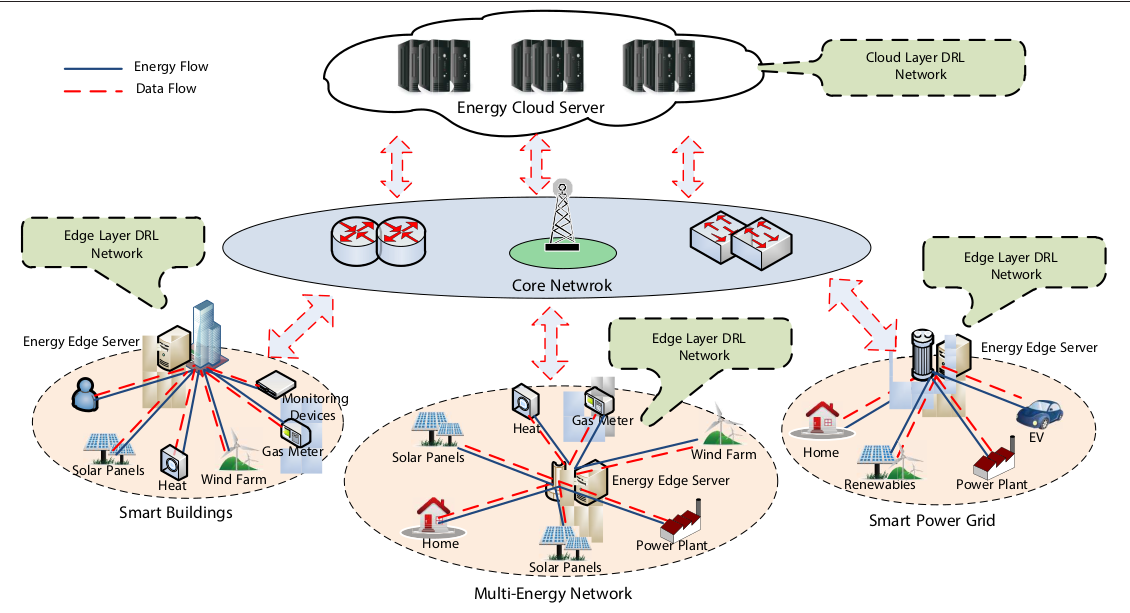
\includegraphics[width=.85\textwidth]{f-2-1.png}}
\caption{معماری کلی مدیریت انرژی یک شهر هوشمند بر پایه اینترنت اشیا}
\end{figure}
